% arara: lualatex: { interaction: nonstopmode, synctex: no }
% arara: makeglossaries
% arara: lualatex: { interaction: nonstopmode, synctex: no }
% arara: lualatex: { interaction: nonstopmode, synctex: no }
\documentclass[a4paper,12pt,chapterprefix=false,bibliography=totoc,listof=totoc,]{scrreprt}

\usepackage{latex-style}

%%%%%%%%%%%%%%%%%%%%%%%%%%%%%%%%%%%%%%%%%%%%%%%%%%%%%%%%%%%%%%%%%%%%%%%%%%%%%%%
%% Linkeinstellungen
%%%%%%%%%%%%%%%%%%%%%%%%%%%%%%%%%%%%%%%%%%%%%%%%%%%%%%%%%%%%%%%%%%%%%%%%%%%%%%%

\hypersetup{
    colorlinks=true,
    linkcolor=blue,
    filecolor=magenta,      
    urlcolor=cyan,
}

\setlength{\parindent}{0pt}

%%%%%%%%%%%%%%%%%%%%%%%%%%%%%%%%%%%%%%%%%%%%%%%%%%%%%%%%%%%%%%%%%%%%%%%%%%%%%%%

% arara: halt
\newabbreviation{k8s}{K8S}{Kubernetes}
\newabbreviation{aws}{AWS}{Amazon Web Services}
\newabbreviation{tbd}{TBD}{To be determined}
\newabbreviation{na}{N/A}{Not applicable}
\newabbreviation{dto}{DTO}{Data Transferable Object}
\newabbreviation{stc}{STC}{Subject to change}
\newabbreviation{gcs}{GCS}{Google Cloud Services}
\newabbreviation{ucd}{UCD}{Use Case Diagramm}

\makeglossaries

\begin{document}	
\begin{flushright}
GameBase
\\
Software Architecture Documentation
% \\
% For <Subsystem or Feature>
\bigbreak
Version 1.0
\end{flushright}
\chapter*{Revision History}
\begin{table}[H]
	\centering
	\everyrow{\hline}
	\begin{tabu} to \textwidth {|X[c]|X[c]|X[c]|X[c]|}
		Date & Version & Description & Author\\
		12/02/2019 & 0.1 & Create initial template & Stefan Lukas \\
		12/02/2019 & 0.5 & Create initial architecture documentation & Norman Gehrsitz \\
		% <mm/dd/yyyy> & <x.x> & <details> & <name>\\
	\end{tabu}
	\label{tab:rev-hist}
\end{table}

\tableofcontents

\chapter{Introduction}
%[The introduction of the Software Architecture Document provides an overview of the entire Software Architecture Document. It includes the purpose, scope, definitions, acronyms, abbreviations, references, and overview of the Software Architecture Document.]

\section{Purpose}
% [This section defines the role or purpose of the Software Architecture Document, in the overall project documentation, and briefly describes the structure of the document. The specific audiences for the document is identified, with an indication of how they are expected to use the document.]
This document provides a comprehensive architectural overview of the system, using a number of different architectural views to depict different aspects of the system. It is intended to capture and convey the significant architectural decisions which have been made on the system.

\section{Scope}
% [A brief description of what the Software Architecture Document applies to; what is affected or influenced by this document.]
This document describes the technical architecture of the GameBase project, including the Go Backend as well as the Angular Frontend.

\section{Definitions, Acronyms and Abbreviations}
\printabbreviations[title={}]

\section{References}
% [This subsection provides a complete list of all documents referenced elsewhere in the Software Architecture Document. Identify each document by title, report number (if applicable), date, and publishing organization. Specify the sources from which the references can be obtained. This information may be provided by reference to an appendix or to another document.]
\begin{table}[H]
	\centering
	\everyrow{\hline}
	\begin{tabu} to \textwidth {|X[c]|X[c]|X[c]|}
		\textbf{Title} & \textbf{Date} & \textbf{Author} \\
		\href{https://gitlab.tandashi.de/GameBase}{Git Repository} & 10/23/2019 & GameBase \\
		\href{https://youtrack.gahr.dev}{YouTrack} & 10/23/2019 & GameBase \\
		\href{https://gahr.dev}{Blog} & 10/23/2019 & GameBase \\
		\href{https://www.docker.com/}{Docker} & 10/23/2019 & Docker Inc. \\
		\href{https://cloud.google.com/}{Google Cloud Services} & 10/31/2019 & Google Ltd. \\
	\end{tabu}
	\label{tab:references-tabview}
\end{table}

\section{Overview}
% [This subsection describes what the rest of the Software Architecture Document contains and explains how the Software Architecture Document is organized.]
The next chapters provide information from different perspectives about the system architecture chosen to fulfill the software requirements.

\chapter{Architectural Representation}
% [This section describes what software architecture is for the current system, and how it is represented. Of the Use-Case, Logical, Process, Deployment, and Implementation Views, it enumerates the views that are necessary, and for each view, explains what types of model elements it contains.]
%Our architecture uses the classical MVC Pattern for the Angluar Frontend as well as the Go backend. To reduce the implementation effort of a sharing the Model(representation of the Kubernetes Data) we use swagger.io.
%This is a visual example of our overall Model:
Our architectures use the following design patterns:
\begin{itemize}
	\item Backend: \gls{mvc}
	\item Frontend: A mix of \gls{mvc} and \gls{mvvm}
\end{itemize}
To provide an easy maintainable shared \gls{dto} of objects to be used in \gls{rest} requests, we use \textit{OpenAPI Specification}. In addition, the backend uses \gls{k8s} for user management and game server deployments.
%TODO PNG ????


\chapter{Architectural Goals and Constraints}
% [This section describes the software requirements and objectives that have some significant impact on the architecture; for example, safety, security, privacy, use of an off-the-shelf product, portability, distribution, and reuse. It also captures the special constraints that may apply: design and implementation strategy, development tools, team structure, schedule, legacy code, and so on.]
By using a \gls{mvc} architecture for both the front- and backend we gain various benefits, like productivity improvements by auto-generating the code for our model implementation in Go and Angular.
\section{Frontend}
For Angular, its design pattern is not strictly set. It is said that it applies \gls{mvc} pattern, but also something of \gls{mvvm} pattern. For this section, we stick to the \gls{mvc} pattern.
\begin{itemize}
	\item Model: \gls{dto} defined in \textit{OpenAPI Specfication} file
	\item View: HTML + CSS in the browser
	\item Controller: Handles incoming interaction of view, updates details if needed and partially validates user input to be sent to the backend
\end{itemize}
\section{Backend}
Our Go Backend also leverages the advantages of a \gls{mvc} design.
\begin{itemize}
	\item Model: \gls{dto} defined in \textit{OpenAPI Specification} file
	\item View: JSON responses
	\item Controller: gin HTTP Request Controller and \gls{k8s} access logic
\end{itemize}
\chapter{Use-Case View}
% [This section lists use cases or scenarios from the use-case model if they represent some significant, central functionality of the final system, or if they have a large architectural coverage—they exercise many architectural elements or if they stress or illustrate a specific, delicate point of the architecture.]
This is the \gls{ucd} of our project:
\begin{figure}
	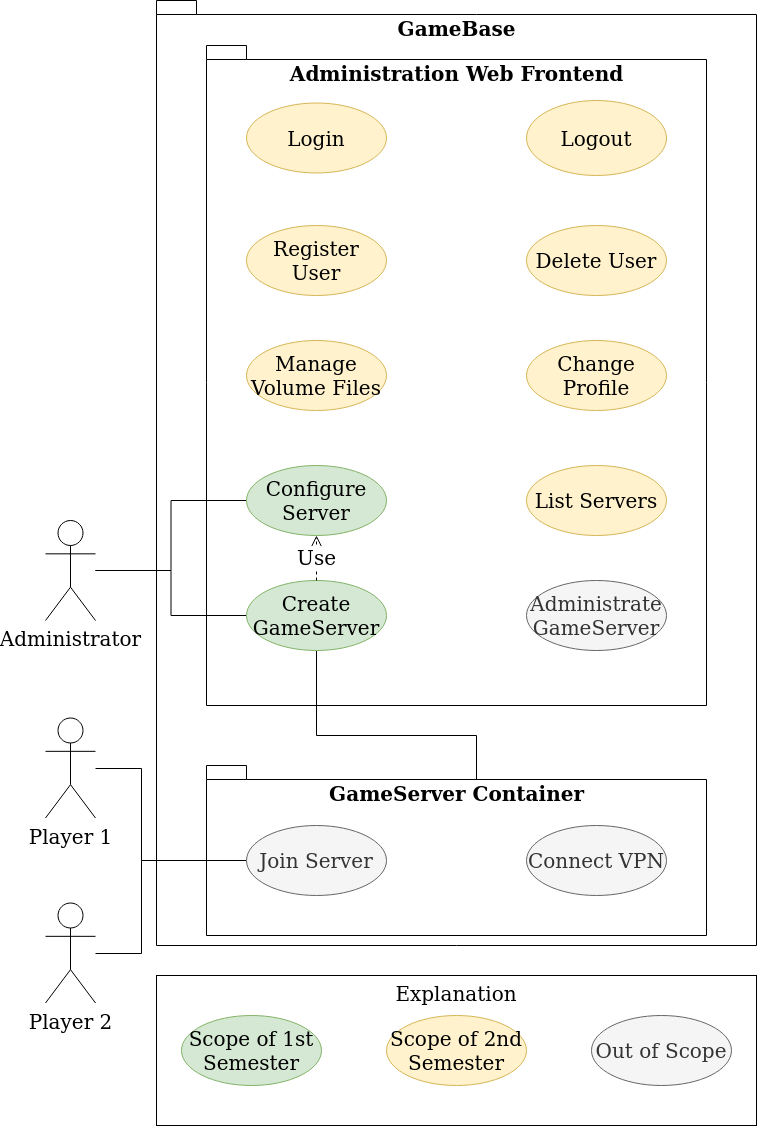
\includegraphics[width=\textwidth]{diagramms/Use_Case_Diagramm.png}
	\label{fig:ucd}
\end{figure}

\section{Use-Case Realizations}
% [This section illustrates how the software actually works by giving a few selected use-case (or scenario) realizations, and explains how the various design model elements contribute to their functionality.]
This section describes an exmplary realization of the use-case \textit{List Servers}.
\subsection{Requirements}
\begin{itemize}
	\item A \gls{rest} endpoint which returns an array of game servers that are available to the server
	\item A \gls{dto} which represents one server
	\item A list on the frontend to display the results
	\item Check authentication of user
	\begin{itemize}
		\item If they are logged in, they can see the list.
		\item Or else the frontend redirects them to the login screen.
	\end{itemize}
\end{itemize}
\subsection{Realization}
\subsubsection{OpenAPI Specification}
This step is necessary as it's required to define an \gls{rest} endpoint for data transfer. Inside of the \gls{yaml} file, we can specify endpoints with their authentication header, request path, request method and responses at ease.
In addition, responses can have references to so called \textit{schemes} which describes a response in general. Both \gls{rest} client and server ship these as possible \gls{dto}s.
Afterwards, both frontend and backend can generate client and server respectively by using the update \gls{yaml} file.
\subsubsection{Frontend}
\paragraph{View}
This use-case uses the \textit{Dashboard} view. \textit{Nebular}'s accordion components consists of two view components: Header and Body. The header can be used as a very concise description of a game server, including:
\begin{itemize}
	\item Server ID
	\item Server name
	\item Server status
	\item Control panel for restart, stop, start and settings actions
\end{itemize}
The body contains detailed information about a game server:
\begin{itemize}
	\item Server description
	\item Template path
	\item Port allocation
	\item Memory allocation
	\item Restart behavior
	\item Startup arguments
	\item Button \enquote{\textit{Delete container}}
\end{itemize}
Each individual accordion item are added to an accordion list.

\paragraph{Controller}
It handles \gls{rest} requests for
\begin{itemize}
	\item Fetching game server details
	\item Starting, stopping and restarting game servers
\end{itemize}
If the user chooses to access the server settings, the corresponding handler function set for a button in the view is triggered, redirecting the user to the settings page.
However, when it comes to checking authentication, the controller for this \textit{Dashboard} component has no effect on it whatsoever. The route to the \textit{Dashboard} is added to Angular Routing. In Angular Routing, routes can be a child entry of a so-called \textit{guard}. A \textit{guard} represents e. g. an interceptor. In this case, an HTTP interceptor exists which checks if the user is authenticated or not before proceeding to the page.

\subsubsection{Backend}
% TODO @ Backend!
As we use the Gin server framework for our backend, incoming requests are dispatched to their request handlers by an automatically generated server. The initial request handler initiates the sequential processing of the request through specialized handlers. Each handler does only one thing, passing any remaing work to the next handler.

There are four request handlers:
\begin{itemize}
	\item The initial request handler creates the chain of request handlers following the Chain of Command design pattern
	\item The \enquote{authentication} request handler checks if the request correctly authorized
	\item The \enquote{parser} request handler parses request data
	\item The \enquote{\gls{k8s} controller} request handler queries the kubernetes cluster to fulfill the request 
\end{itemize}

\chapter{Logical View}
% [This section describes the architecturally significant parts of the design model, such as its decomposition into subsystems and packages. And for each significant package, its decomposition into classes and class utilities. You should introduce architecturally significant classes and describe their responsibilities, as well as a few very important relationships, operations, and attributes.]

\section{Overview}
% [This subsection describes the overall decomposition of the design model in terms of its package hierarchy and layers.]
% TODO: Add Frontend diagram

\subsection{Backend}
% Generated with: goplantuml -recursive -show-aggregations -show-implementations -show-compositions -aggregate-private-members .
% https://plantuml.gahr.dev/png/xLhTRzis47_tNq6uBtRcUDrMj2zPWCnfsc3zCE8aUoYAG94PMwiaQXILfDZwl-yewkCaKg8a1qEA9Iz9oBlV7O_77u-aGYUWSUIubB28XaxaaRz717vStubZylhUfP7mM4WE3iXaDJlwAt42XtiXdPB3mqnK_ln0JjSa5j2pGMsbkjPrJ8NZ-N7UaVPyGvRVW5yB5e9GI3dySUDj4kvqSoN7RiR8993E6OrPmbtQfbN8z74tTyRgzOhoMye_090fMh7BlKeeUxXGZitgn3aD8jyHTEc8hUx6ad4Haq-VvU_tJXHLUz_JWF6ln0l5Bp_ZSGc7YoGwufjOHmJNPFTlTElSUepN_yUv5Dvwd8K13SMbms4eDp1MuZAVyL-l_OGU1avqyADiFFoap7pk5AbZ6ldiguGT5frsT1YyIE9XgoVJLRzGUtKrD4yxKf52Ah-ATDmjVDTEJ2zYokqZCoVqwm2yC2GOuDynRWZ66-xSEf0QbR1diy9MrELK74F_PBhBoDuA4PtHln98mYLdi61Y45ji8RIsSUwJaDwBjqwuzY4esn8dQyB-lcCRBvouP0z-pUNKWUQKL0LO8jeapkZ6YmNbhIWWaITit2RuXWgLOsr2UMQLkTOchHPL9z6K7ZfAigYJO4OY7JtrgUWsg8je3Q6KMG_9SUFvL1VMCWenfNsf0AnWaBZ57tWPiJMLO1gz5gwZNisDCyWdEdIjlgTYozQcnIeW1GrxUvRp9qde4XaVzB_kMZSMQU2BayJtpKwVio-qUQ-KHjDbEDXodQcC9h8yiHkHmk4WeaHcyZORQpPuMK1QlVte6xBX0xrhjP9JbXs-UL9xxnefQ_70EbcROd-q4xsRCY5iAkHBSWtJ1lGHBrWGiH1g24MJiEAHGdJhcaINbmiaj2xB48DiMQGW5GZghGU5kq5-fRf6I7f34I5EoUrFy-9V9CMfipOKCA1WQ1rLDv6BqsEGqtVkOdkPwhKCTCgfDkcjigwGtg5igEzS-GxNO1dnBqWqLQwhgY1OnBnTqQhRBqAYgjztNk09iAGLmGsIO2hzGoaOjkMyT6w849O0B5Harx7G4Q812qi0bdxcg4FMYdM0RIxVLxeusB2K_tM3jJD0hsAluaeT25o1fXvLiPw6FF32jEm-zm8goxSfsOD9VVb2go3AOdpYudfTzROKz5CosIkPQaOevn2ZDZRBLuUTrKGcQIBUxvJpMjdbZ8Qg9mrYZSX23sftD4rJ558aUkdudfooIHwy9QSttdsnMXIqDZteT72KY2suxhcEOFpXpXZxE3w-1nPW2FMcfoF9ztyaaVcJpjsInQA38CoXGd-uSmvm7EKtyW9HpqXIoTwdd7mw9ZSSar7g_8wOFHIS-JxTdHdHJkRhIQVlWlAISq_VHlioR2bDxo7DOe7s56-jLrMmRq8rGa_NcVjQv2PAPKQGSzDA-HwxZXRn6RH7FcmoSLvcNZFcFwsr__rQMyfiUwexdlBklyYxUXxOBu8okRrISwwQOYfgPNv9h7Ak9wwubsSMwKf9Wc7nr9aJxwJ2yiM1gW6v6-gC90dYzacx0PKTnIL6HmlvDaKCUrG7atAQvR3YNiE2FDfGKTbvjCFJEQIRoWqrCBf-63kM8JqYatzuOlinlJI9Xrk774hXCo1vMNU16wpUdULrm70FLDjPhN2eJ_Y2Kna6vdx9xohKMrnNo-ZIUqRae-BB5t4AW1OGZ5w16WQgx4iYsi5k8ZT1_AhPpUeE5jKOpxz6b1Hsv7-pJ48-PVQvZ6ftDxtRkt4IFxyZEN9TbeJYD70sT9du_k2H59Onh9b7TxVHC3grClh1PpbMudO8eIt9A7gSCEQKwQO9jWex6ghx6rBnGpx2vW1Keraec2UhprWb8XveuvRJ3xJXygpj_j5UKMItVeRBJdrw1jxkjTvaFbOFbvUBn-fQnYsFmhti4xbvyL0ldJgVaMSd9wzUFN-UkfJvP5AhltRqr9Pl-75F9VJzaLr9SjR2TxoWouTYydtzegnqQu_P3I-riilyj2jx6bwhlut6whLIhV8nsTlV9-DyX6s4C4uro-LdLqMogUwIybWUBqDnoVmae6bux32mdfH-bhrsZLnmDFxpJiXf2zSENwlPg6cNqpGUZOfM_Lm-9WV_OBscTuVnG13JJTrGB7KJWSVJ_0ms9WoZM3-z73yeQF4nPIVOKhgAZrwKTyAfKKeJbgA1pcFi1PCrbYhDNz7LD0qPCZ96g1QxZ7sHSCgDcLZjYoCaXUuhQf26ps2GNdaiggbPk6U8VeM0XW0ewXcYMLAGhftVBkmQWEuuba1q1seAI7S4FJ2DLDeZmMrCMeKo-3qKwW6zgj_fcO4oSk_XXOQhT4qNWNBFkBgwJZnVUE7LrLpL3cFoR3utKePLLgTKguf6WPy-PunKHKuhkF6_
\begin{sidewaysfigure}[ht]
    \centering
    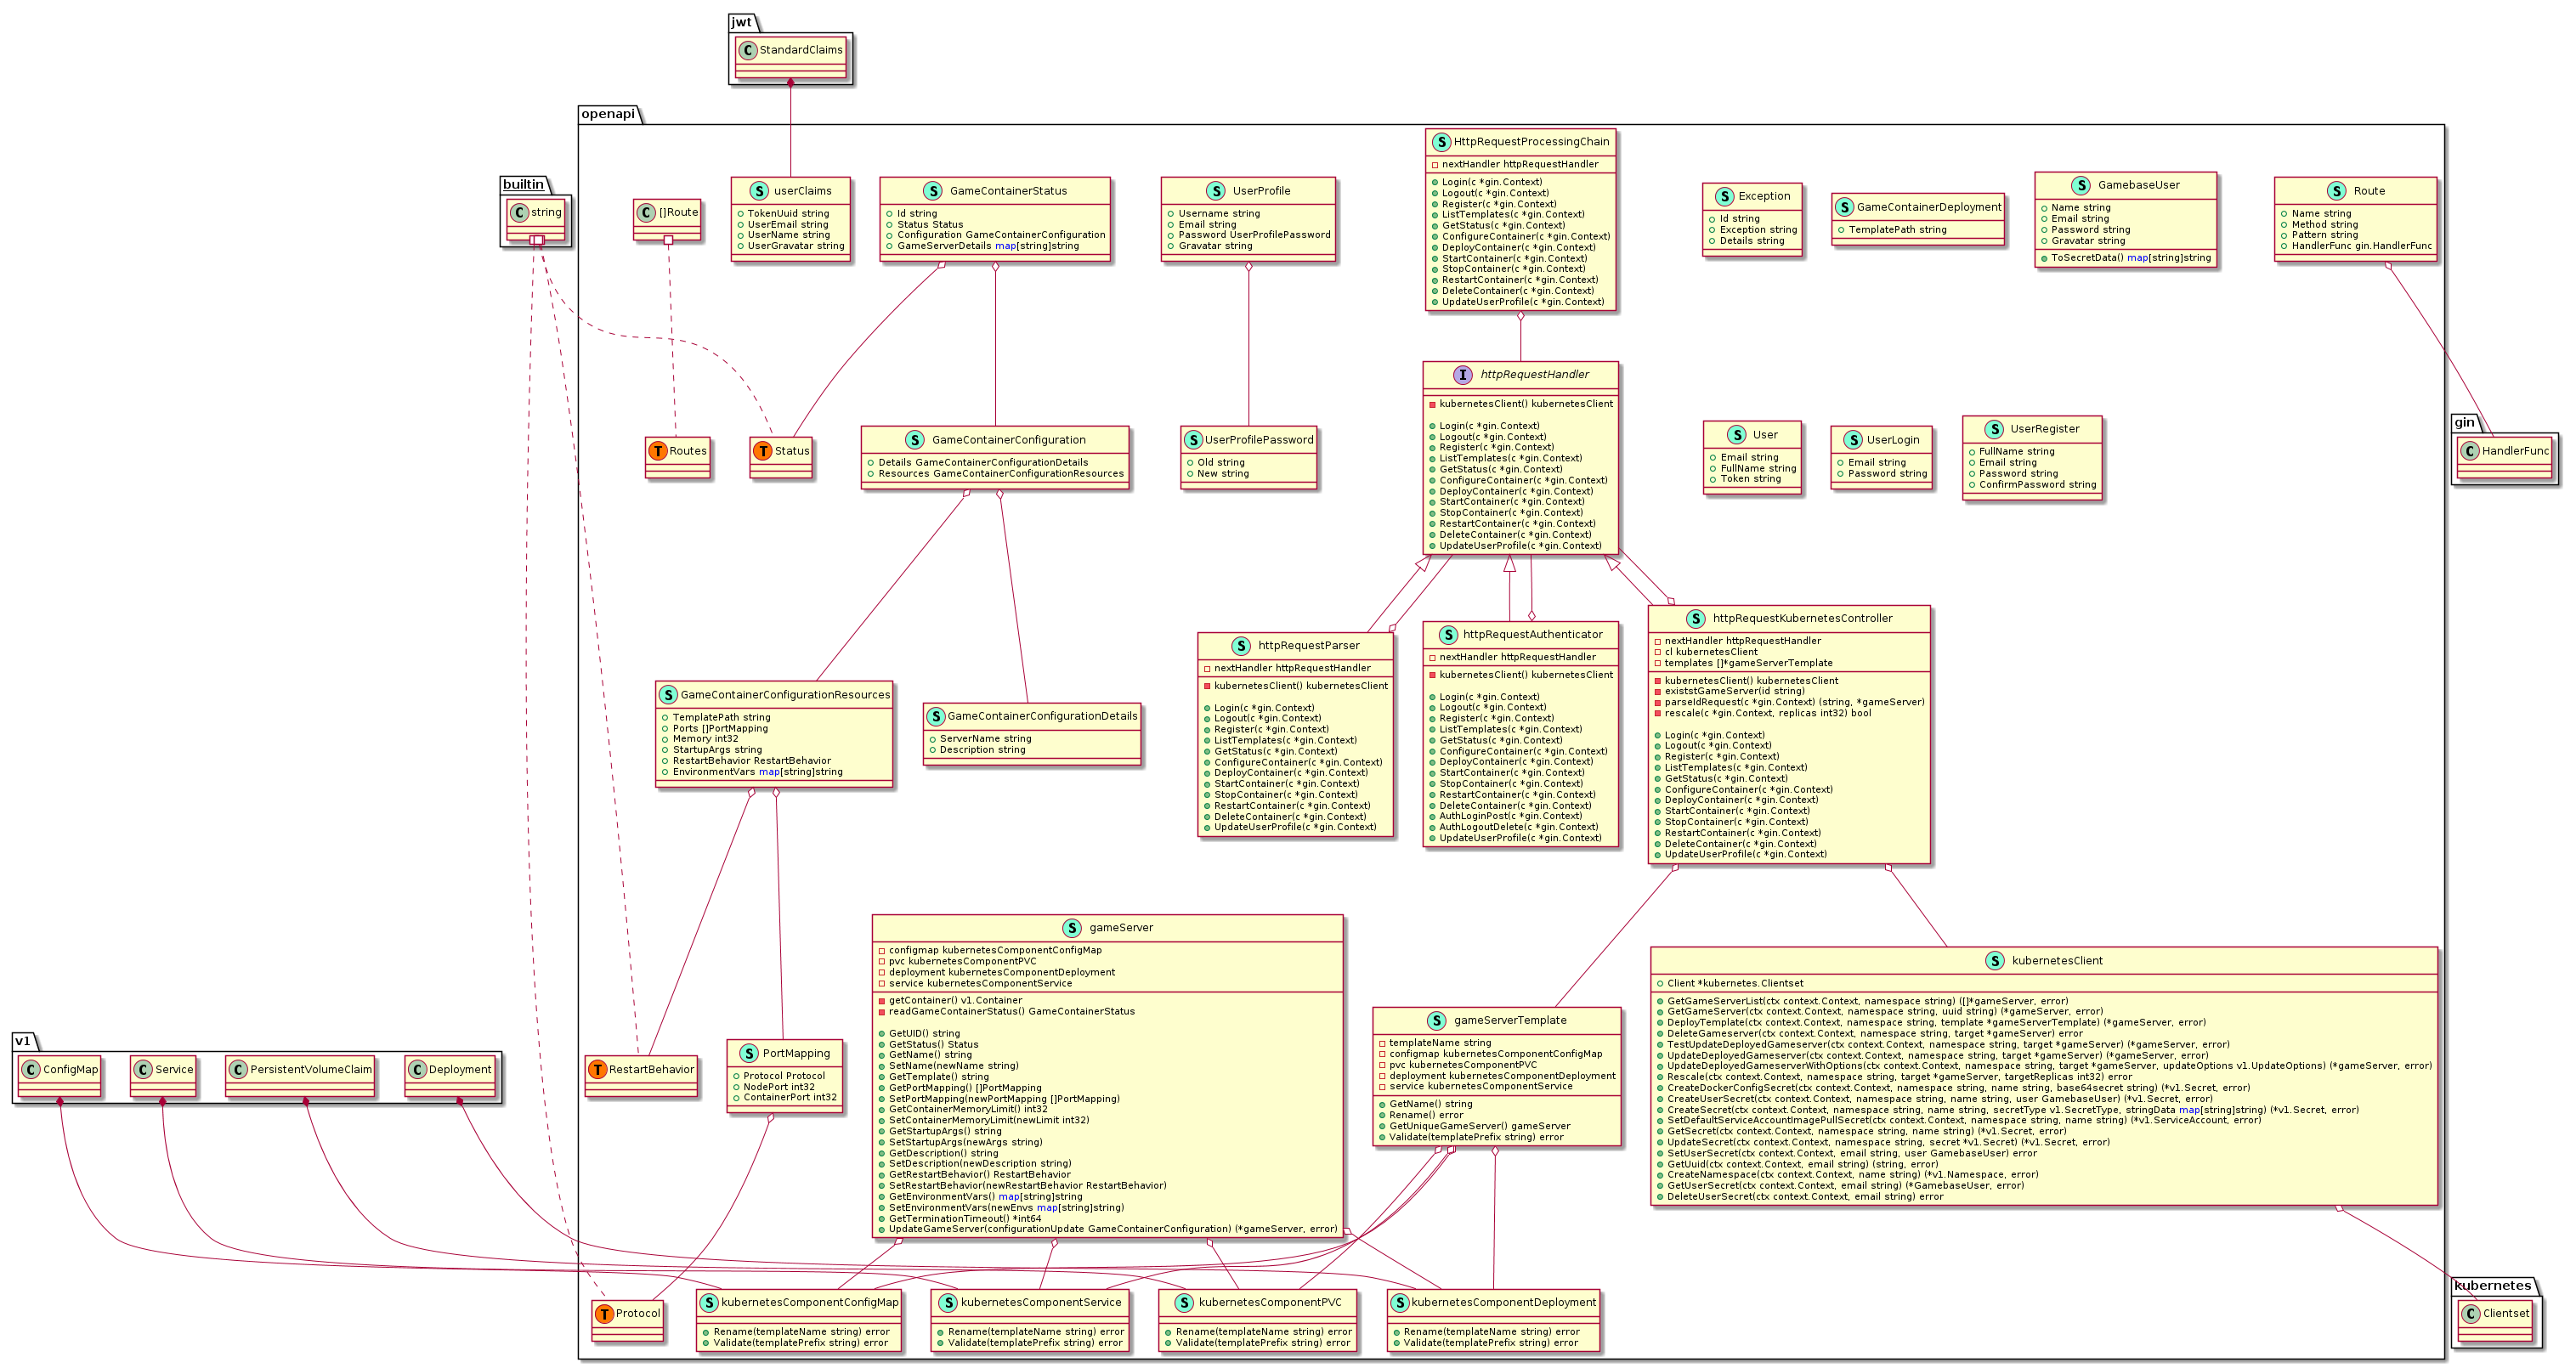
\includegraphics[width=\textwidth]{diagramms/BackendOverview.png}
    \label{fig:backend-overview}
\end{sidewaysfigure}
\clearpage

\section{Architecturally Significant Design Packages}
% [For each significant package, include a subsection with its name, its brief description, and a diagram with all significant classes and packages contained within the package.
\subsection{Frontend}
% TODO Frontend diagram
The \texttt{e2e} directory represents E2E tests with \textit{Protractor}. They cover Gherkin feature tests. The source code is available in \texttt{src/app}. Each folder inside represents a component in Angular, except for \texttt{mock}, \texttt{rest-client} \texttt{binding} and \texttt{global.ts}. \\
\texttt{mock} provides a mocked \textit{OpenAPI} \gls{rest} client (located in \texttt{mock/mockapi/services}) hat is used in Karma unit tests. Meanwhile it should return responses like expected from backend, it doesn't do any changes to mocked data. If necessary, the corresponding mock class has to be adjusted. Another disadvantage is that the mock service is not generated - whenever the API changes, the new functions available have to implement if they are needed for testing. \\
\texttt{rest-client} contains generated \gls{rest} client code by \texttt{ng-openapi-gen}. However, the contents of that directory is not committed, as the client code generated either on the developer workstation or while building in CI/CD. \\
\texttt{binding} provides models that can be used multiple times. \\
\texttt{global.ts} is a collection of util classes that can be used across the whole frontend project. \\
The \texttt{vendor} directory represents dependencies that cannot be pulled from e. g. \texttt{npm} thus are most likely pulled as submodule from a Git repository. Currently, it only contains the \textit{OpenAPI Specification} \gls{yaml} for code generation. Whenever an update to it occurs, the submodule has to be updated manually.

\subsection{Backend}
We were unable to clearly separate the different components into distinct directories for two tooling-related reasons which were out of our control. They are, however, separated on a best-effort basis. The diagram \ref{fig:backend-overview} gives a graphical representation of the backend components.

The separation into different components is thus only logical in nature.
\texttt{main.go} is the main entry point of the backend application. It starts the server and prepares it for accepting incoming requests. \\
The files \texttt{openapi/routers.go} is automatically generated and dispatches to the automatically generated request handler functions in \texttt{openapi/api\_*.go} \\
The files \texttt{openapi/api\_*.go} contain the automatically generated request handler functions. These solely forward requests to our request handling pipeline. \\
The files \texttt{openapi/model\_*.go} contain the automatically generated models which are used as request or response messages. \\
The files \texttt{openapi/kubernetes\_*.go} contain Kubernetes specific functionality. They serve as an abstraction layer over the Kubernetes API and help reduce the complexity of our request handlers. \\
The files \texttt{openapi/gameserver*.go} are a higher-level abstraction over the Kubernetes API specialized to maintain game servers in a Kubernetes cluster.  \\
The files \texttt{openapi/authentication*.go} provides helper functions for user authentication. \texttt{openapi/user.go} provides an additional model for this purpose. \\
The files \texttt{openapi/http\_request*.go} are the stages in our request handling process. Each of these files contains a request handler. They are loosely coupled to each other and tightly coupled to our abstractions over the Kubernetes API and the authentication helpers.

\chapter{Process View}
% [This section describes the system's decomposition into lightweight processes (single threads of control) and heavyweight processes (groupings of lightweight processes). Organize the section by groups of processes that communicate or interact. Describe the main modes of communication between processes, such as message passing, interrupts, and rendezvous.]
\gls{na}

\chapter{Deployment View}
% [This section describes one or more physical network (hardware) configurations on which the software is deployed and run. It is a view of the Deployment Model. At a minimum for each configuration it should indicate the physical nodes (computers, CPUs) that execute the software and their interconnections (bus, LAN, point-to-point, and so on.) Also include a mapping of the processes of the Process View onto the physical nodes.]
This is our deployment view including the Kubernetes cluster which is being accessed from our backend.
\begin{figure}
	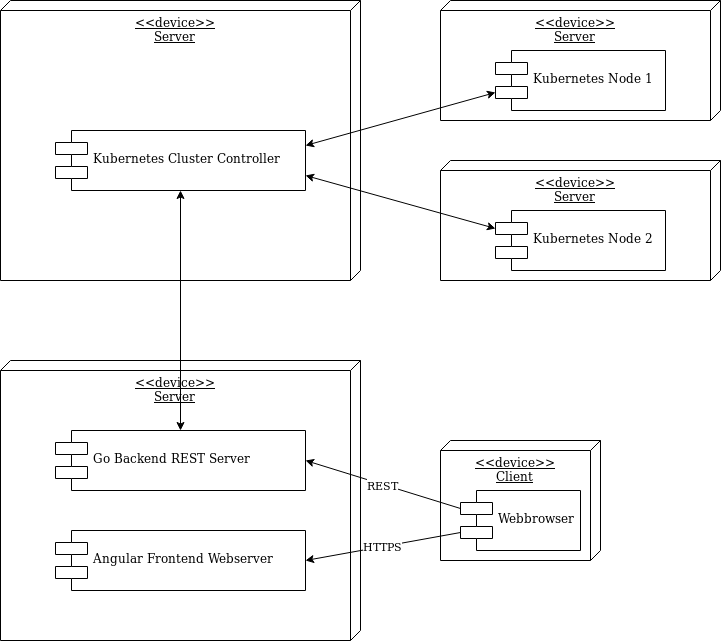
\includegraphics[width=\textwidth]{diagramms/DeploymentView.png}
	\label{fig:ucd}
\end{figure}

\chapter{Implementation View}
% [This section describes the overall structure of the implementation model, the decomposition of the software into layers and subsystems in the implementation model, and any architecturally significant components.]
\gls{na}

%\section{Overview}
% [This subsection names and defines the various layers and their contents, the rules that govern the inclusion to a given layer, and the boundaries between layers. Include a component diagram that shows the relations between layers. ]
%\gls{na}

%\section{Layers}
% [For each layer, include a subsection with its name, an enumeration of the subsystems located in the layer, and a component diagram.]
%\gls{na}

%\chapter{Data View (optional)}
% [A description of the persistent data storage perspective of the system. This section is optional if there is little or no persistent data, or the translation between the Design Model and the Data Model is trivial.]

\chapter{Size and Performance}
% [A description of the major dimensioning characteristics of the software that impact the architecture, as well as the target performance constraints.]
Our software acts as a middleman between the users frontend and a \gls{k8s} cluster. As such performance mainly depends on the \gls{k8s} cluster where containers are deployed to. Furthermore, Go is a well optimized and multitasking oriented language. So even having multiple users send configuration requests to our backend should be no concern regarding performance.

\chapter{Quality}
% [A description of how the software architecture contributes to all capabilities (other than functionality) of the system: extensibility, reliability, portability, and so on. If these characteristics have special significance, such as safety, security or privacy implications, they must be clearly delineated.]
We use \textit{GitLab} both as Git repository remote and CI/CD. The CI is triggered if the following conditions are fulfilled:
\begin{itemize}
	\item Push to \texttt{dev} or other branches
	\item Tag release after branching off from \texttt{master} branch
\end{itemize}

Each pipeline goes through the processes:
\begin{itemize}
	\item Install dependencies and push dependencies as cache to S3 bucket (frontend)
	\item Generate Swagger (\textit{OpenAPI}) client
	\item Verify tests (E2E, Karma, TSLint)
	\item Build \texttt{dev}/\texttt{release}
	\item Check code with \textit{SonarQube Scanner}
	\item Create and publish Docker image
	\item Deploy software
\end{itemize}
Every pipeline can be accessed in either frontend's or backend's project.

To prevent code smells or common bugs, we introduced the usage of \textit{SonarQube} whose scanner is always run in CI pipelines.

\chapter{Supporting Information}
% [The supporting information makes the SRS easier to use.  It includes:
% \begin{itemize}
% 	\item Table of contents
% 	\item  Index
% 	\item Appendices
% \end{itemize}
% These may include use-case storyboards or user-interface prototypes. When appendices are included, the SRS should explicitly state whether or not the appendices are to be considered part of the requirements.]
If you want to reach out to use, feel free to write us an e-mail:
\begin{itemize}
	\item \href{mailto:gahr.leonhard@student.dhbw-karlsruhe.de}{Leonhard Gahr}
	\item \href{mailto:gehrsitz.norman@student.dhbw-karlsruhe.de}{Norman Gehrsitz}
	\item \href{mailto:lukas.stefan@student.dhbw-karlsruhe.de}{Stefan Lukas}
	\item \href{mailto:reis.kevin@student.dhbw-karlsruhe.de}{Kevin Reis}
\end{itemize}

Otherwise, take a look at section \ref{tab:references-tabview} for other possibilities to reach us out.
\end{document}
